\documentclass[12pt,a4paper]{article}
\usepackage[a4paper,top=1.5cm, bottom=1.5cm, left=1.5cm, right=1.5cm]{geometry}
\usepackage[T2A]{fontenc}
\usepackage[utf8]{inputenc}
\usepackage[russian]{babel}
\usepackage{amsmath}
\usepackage{amssymb}
\usepackage{graphicx}
\usepackage{floatrow}
\usepackage{booktabs}
\usepackage{wrapfig}
\usepackage{lipsum}
\usepackage{subcaption}

\newcommand{\figref}[1]{(См. рис. \ref{#1})}
\newcommand{\e}[1]{\text{$\cdot10^{#1}$}}

\title{Лабораторная работа 2.5.1\\ Измерение коэффициента поверхностного натяжения жидкости}
\author{Симанкович Александр \\ Б01-104}
\date{23.03.2022}

\usepackage{float}
\restylefloat{table}

\begin{document}
	\maketitle
	
	\section*{Цель работы}
	
	$\quad$ Измерение коэффициента поверхностного натяжения исследуемой жидкости при разной температуре с использованием известного коэффициента поверхностного натяжениядругой жидкости
	
	Определение полной поверхностной энергиии теплоты, необходимой для изотермического образования единицы поверхности жидкости.
	
	\section*{Оборудование и приборы} 
	$\quad$ Прибор Ребиндера с термостатом, исследуемые жидкости, стаканы.
	
	\section*{Теоретическое введение}
	
	$\quad$ Наличие поверхностного слоя приводит к различию давлений поразные стороны от искривленной границы раздела двух сред. Для сферического пузырька внутри жидкости избыточное давление дается формулой Лапласа
	
	$$\Delta P = P_\text{внутри}-P_\text{снаружи}=2\sigma/r.$$
	
	Эта формула лежит в основе предлагаемого метода определения коэффициента поверхностного натяжения жидкости. Измеряется давление, необходимое для выталкивания в жидкость пузырька газа.
	
	\section*{Экспериментальная установка}
	
	$\quad$  Исследуемая жидкость наливается в сосуд $B$. Дистиллированная вода наливается в сосуд $E$. Сосуды закрыты пробками. Через пробку сосуда, в котором проводятся измерения, проходит полая металлическая игла $С$, нижний конец которой погружен в жидкость, а верхний открыт в атмосферу. Если другой сосуд герметично закрыт, то в сосуде с иглой создается разрежение, и пузырьки воздуха начинают пробулькивать через жидкость. Поверхностное натяжение можно найти по величине разрежения, необходимого для прохождения пузырьков. При приоткрытом кране $\text{К}_1$ из аспиратора $A$ по каплям вытекает вода, создавая разрежение, которое измеряется наклонным спиртовым манометром $М$. Показания манометра, умноженные на зависящий от наклона коэффициент, дают давление в $\text{кгс}/\text{м}^2$. Чтобы пополнить запас воды, достаточно при помощи крана $\text{К}_2$ соединить нижнюю часть аспиратора с атмосферой и предварительно заполненной водой верхней частью. Через рубашку $D$ непрерывно прогоняется вода из термостата для стабилизации температуры исследуемой жидкости.
	
	
	\begin{figure}[h]
		\begin{center}
			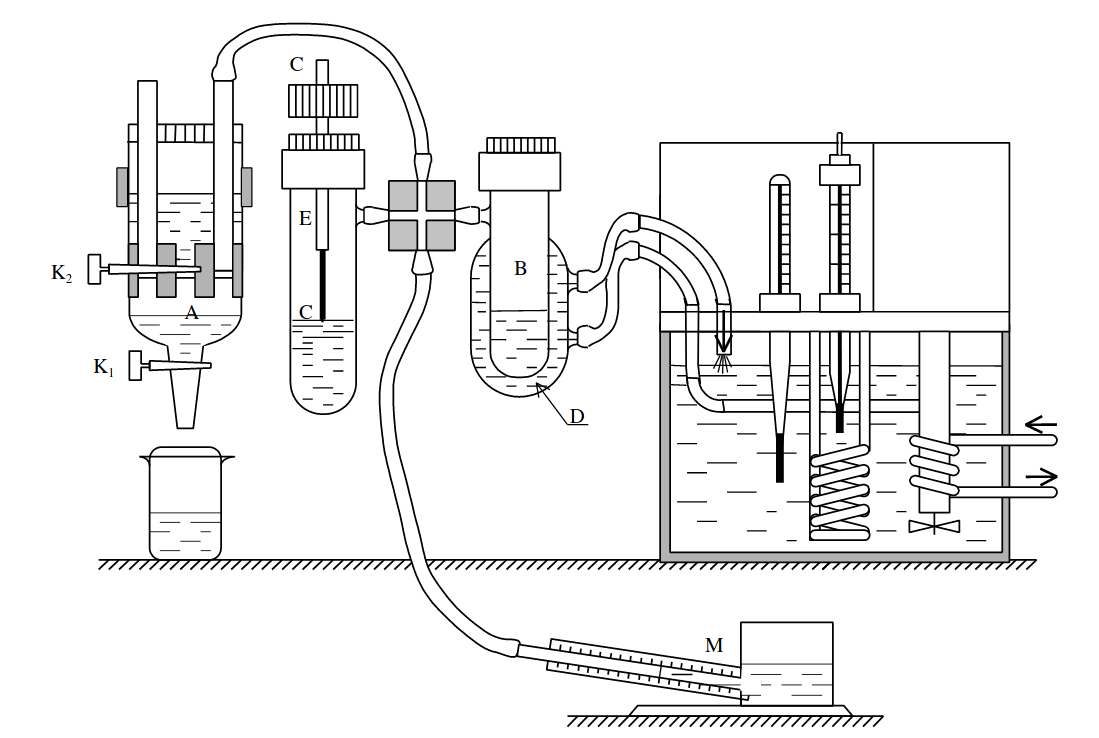
\includegraphics[width=0.9\linewidth]{scheme.png}
		\end{center}
		\caption{Схема установки}
		\label{scheme}
	\end{figure}	
	
	
	\section*{Ход работы}
	
	\subsection*{Спирт}
	
		$\quad \;$ Коэффициент пересчета столба спиртового манометра в давление:
		
		$$K = 0.2 \cdot 9.81 \cdot 0.8095 = 1.588 \; \text{Па}/\text{мм}$$
	
		Поместим иглу в сосуд со спиртом, закроем пробками сосуды, открыв кран аспиратора добьемся пробулькивания пузырьков воздуха.
		
		\begin{table}[h]
			\caption{Давление пробулькивания, спирт, игла на поверхности}
			\begin{tabular}{|l|llllllllll|}
				$h_{eth}$, мм & 46    & 45    & 45    & 45    & 45    & 46    & 46    & 46    & 46    & 46        \\
				$p_{eth}$, Па & 73.06 & 71.47 & 71.47 & 71.47 & 71.47 & 73.06 & 73.06 & 73.06 & 73.06 & 73.06
			\end{tabular}
		\end{table}
	
		$$p = (72.4 \pm 1.4) \; \text{Па}$$
		
		Воспользовавшись табличным значением поверхностного натяжения для спирта:
		
		$$\sigma_{\text{сп}} = (22 \pm 2) \text{мН} / \text{мм}$$
		
		Значения диаметра иглы, измеренные с помощью микроскопа и косвенно:
		
		$$ d_{\text{микр}} = (1.05 \pm 0.05) \; \text{мм} \qquad d_{\text{косв}} = \frac{4\sigma}{p} =  (1.22 \pm 0.11) \; \text{мм} $$
		
	\subsection*{Вода}
	
		$\quad$ Измерим давления, при которых начинается пробулькивание.
		
		\begin{table}[H]
			\caption{Давление пробулькивания, вода, игла на поверхности}
			\begin{tabular}{|l|llllllllll|}
				$h_{surf}, \; \text{мм}$ & 105    & 104    & 103    & 104    & 104    & 105    & 104    & 104    & 104    & 104    \\
				$p_{surf}, \; \text{Па}$ & 166.77 & 165.18 & 163.59 & 165.18 & 165.18 & 166.77 & 165.18 & 165.18 & 165.18 & 165.18
			\end{tabular}
		\end{table}
		
		\begin{table}[H]
			\caption{Давление пробулькивания, вода, игла на глубине}
			\begin{tabular}{|l|llllllllll|}
				$h_{deep}, \; \text{мм}$ & 189    & 189    & 189    & 189    & 189    & 189    & 189    & 189    & 189    & 189    \\
				$p_{deep}, \; \text{Па}$ & 300.18 & 300.18 & 300.18 & 300.18 & 300.18 & 300.18 & 300.18 & 300.18 & 300.18 & 300.18
			\end{tabular}
		\end{table}
	
		$$\Delta h = h_1 - h_2 = (15.0 \pm 0.5) \; \text{мм}$$
		
		$$\Delta h = \frac{p_2 - p_1}{\rho g} = (13.7 \pm 0.3) \; \text{мм}$$
	
		Формула для определения $\sigma$:
		
		$$ \sigma = \frac{pr}{2}$$
		
		Погрешности измерения:
		
		$$\varDelta p = 1.6 \; \text{Па} \qquad \varDelta T = 0.2 \; \text{K} \qquad \varDelta \sigma = \sigma \sqrt{ (\varDelta p / p)^2 + (\varDelta r / r)^2 } = 2 \; \text{Н} / \text{м}$$

\newpage

		Измерим зависимость давления от температуры.
		
		\begin{table}[h]
			\caption{Зависимость $p(T)$}
			\input{T_p_raw.tex}	
		\end{table}
		
		\begin{table}[h]
			\caption{Зависимость $\overline{p}(T)$}
			\input{T_p_sgm.tex}
			
		\end{table}
		
		Построим график.
		
		\begin{figure}[H]
			\includegraphics{sgm_T.pdf}
			\caption{$ \text{Зависимость} \; \sigma(T)$}
		\end{figure}
		
		
		По методу наименьших квадратов, предполагая зависимость линейной ($y = ax + b$):
		
		\begin{table}[h]
			\caption{Параметры регрессии $\sigma (T)$}
			\begin{tabular}{rrrrrrrrr}
				\hline
				$\overline{x}$ & $\sigma_x^2$ & $\overline{y}$ & $\sigma_y^2$ & $r_{xy}$ & $a$ & $\Delta a$ & $b$ & $\Delta b$ \\
				4.62e+01 & 9.22e+01 & 48.62 & 1.04e+00 & -9.46e+00 & -0.10 & 0.02 & 53.37 & 0.91 \\
				\hline
			\end{tabular}
		\end{table}
	
\newpage

		Также построим графики:
		
		1) теплоты образования единицы поверхности жидкости $q = - T \frac{d\sigma}{dT}$.
		
		2) поверхностной энергии $U$ единицы площади $F$: $\frac{U}{F} = \sigma - T \frac{d\sigma}{dT}$.
		
		\begin{table}[h]
			\caption{Зависимости $q(T), \; U/F(T)$}
			\input{T_q_U_F.tex}
		\end{table}
				
		\begin{figure}[H]
			\includegraphics{q_T.pdf}
			\caption{$ \text{Зависимость} \; q(T)$}
		\end{figure}
		
		\begin{figure}[H]
			\includegraphics{U_F_T.pdf}
			\caption{$ \text{Зависимость} \; U/F \;(T)$}
		\end{figure}
		
	\section*{Вывод}
	
		$\quad$ Данные, собранные в эксперименте, плохо подчиняются теоретической модели. В процессе эксперимента было обнаружена негерметичность установки (при закрывании аспиратора происходило падение давления). Предполагаются корректными последние 4 точки на зависимости. Для наглядности на графике $\sigma (T)$ приведены точки, при которых была течь.
		
		Значение $\sigma_{\text{табл}} = 73 \; \text{мН}/\text{м}$ не сходится с экспериментальным $\sigma_{\text{эксп}} = 48 \; \text{мН}/\text{м}$. Отклонение может возникнуть вследствие попадания спирта в пробирку с водой из-за нетщательной просушки иглы в предыдущих экспериментах (спирт имеет $\sigma_{\text{сп}} = 22 \; \text{мН}/\text{м}$, поэтому поверхностное натяжение смеси ниже).
		
		Значение $(d\sigma/dT)_{\text{табл}} = - 0.15 \; \frac{\text{мН}}{\text{м} \cdot \text{K}}$ (рассчитано по правилу Этвёша) не сходится с экспериментальным $(d\sigma/dT)_{\text{эксп}} = - (0.10 \pm 0.02) \; \frac{\text{мН}}{\text{м} \cdot \text{K}}$. Предположительно ошибка связана с малым количеством экспериментальных данных и с попаданием спирта в пробирку с водой.
	
\end{document}